% Title: gl2ps_renderer figure
% Creator: GL2PS 1.4.0, (C) 1999-2017 C. Geuzaine
% For: Octave
% CreationDate: Thu Nov 28 11:10:23 2019
\setlength{\unitlength}{1pt}
\begin{picture}(0,0)
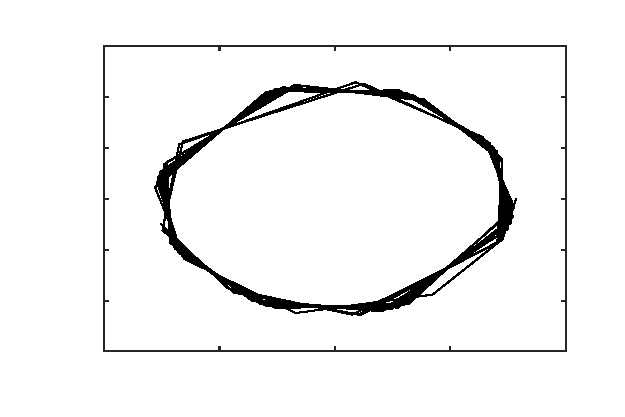
\includegraphics{../Report/img/faseHamilton-inc}
\end{picture}%
\begin{picture}(300,200)(0,0)
\fontsize{10}{0}
\selectfont\put(49.989,24){\makebox(0,0)[t]{\textcolor[rgb]{0.15,0.15,0.15}{{-2}}}}
\fontsize{10}{0}
\selectfont\put(105.367,24){\makebox(0,0)[t]{\textcolor[rgb]{0.15,0.15,0.15}{{-1}}}}
\fontsize{10}{0}
\selectfont\put(160.745,24){\makebox(0,0)[t]{\textcolor[rgb]{0.15,0.15,0.15}{{0}}}}
\fontsize{10}{0}
\selectfont\put(216.122,24){\makebox(0,0)[t]{\textcolor[rgb]{0.15,0.15,0.15}{{1}}}}
\fontsize{10}{0}
\selectfont\put(271.5,24){\makebox(0,0)[t]{\textcolor[rgb]{0.15,0.15,0.15}{{2}}}}
\fontsize{10}{0}
\selectfont\put(45,31.4757){\makebox(0,0)[r]{\textcolor[rgb]{0.15,0.15,0.15}{{-0.06}}}}
\fontsize{10}{0}
\selectfont\put(45,55.8964){\makebox(0,0)[r]{\textcolor[rgb]{0.15,0.15,0.15}{{-0.04}}}}
\fontsize{10}{0}
\selectfont\put(45,80.3172){\makebox(0,0)[r]{\textcolor[rgb]{0.15,0.15,0.15}{{-0.02}}}}
\fontsize{10}{0}
\selectfont\put(45,104.738){\makebox(0,0)[r]{\textcolor[rgb]{0.15,0.15,0.15}{{0}}}}
\fontsize{10}{0}
\selectfont\put(45,129.159){\makebox(0,0)[r]{\textcolor[rgb]{0.15,0.15,0.15}{{0.02}}}}
\fontsize{10}{0}
\selectfont\put(45,153.579){\makebox(0,0)[r]{\textcolor[rgb]{0.15,0.15,0.15}{{0.04}}}}
\fontsize{10}{0}
\selectfont\put(45,178){\makebox(0,0)[r]{\textcolor[rgb]{0.15,0.15,0.15}{{0.06}}}}
\fontsize{11}{0}
\selectfont\put(160.745,11){\makebox(0,0)[t]{\textcolor[rgb]{0.15,0.15,0.15}{{Posición $\theta$}}}}
\fontsize{11}{0}
\selectfont\put(16,104.738){\rotatebox{90}{\makebox(0,0)[b]{\textcolor[rgb]{0.15,0.15,0.15}{{Momento $p_{\theta}$}}}}}
\fontsize{11}{0}
\selectfont\put(160.745,188){\makebox(0,0)[b]{\textcolor[rgb]{0,0,0}{{Retrato fase $\theta / p_{\theta}$}}}}
\end{picture}
